
\section{Client Overview}
\label{sec:client_des}

\begin{figure*}[!t]
   \centering
      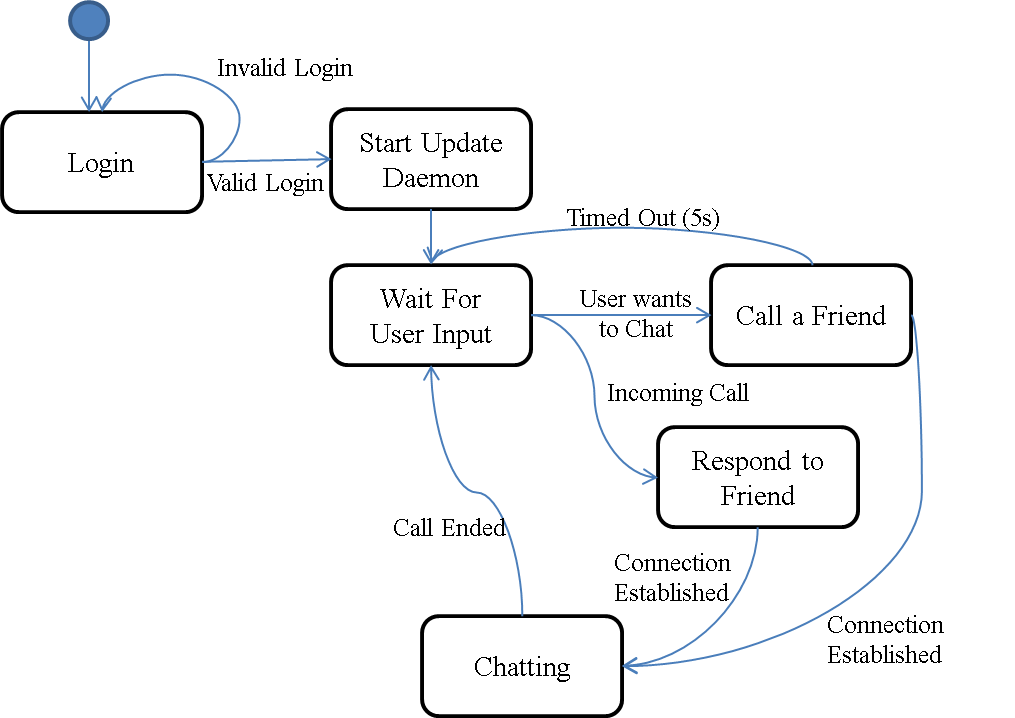
\includegraphics[width=0.8\textwidth]{pics/Client_StateDiagram}
   \caption{Client State Diagram demonstrating the general flow on the client-side.}
\label{fig:client_state_diag}
\end{figure*}

The client application is the core of the voice chatting system. It initiates all
communication with the server in order to receive the user's personal 
information, which includes a friends list. For the purposes of this paper, a
friend is a separate client who appears on the list of people a user can call. The application currently
does not allow users to add friends at run-time.  Once the 
user logs into the server,
the client can make outgoing calls or answer incoming calls.  The
application only supports one-to-one chatting, and has a notification system that 
indicates when a friend is calling while the user is chatting with another client.  

The client handles all audio transmissions between itself and another user
and also manages the setup and teardown of the transport protocol used to
communicate between two clients.  Each client is fitted with a transport protocol
object that handles all the layer three calls which send and receive data between
two clients using sockets.  The specific transport layer protocol is specified
as a command-line parameter when the application is started.
The three options are DCCP, UDP, and TCP. Because clients can both initiate
outgoing calls and accept incoming calls, both a \textit{server} and a
\textit{client} model must be present on each client's computer in order to
monitor a socket for incoming calls as well as open a new socket for outgoing calls.  Fig.~\ref{fig:client_state_diag} gives 
a state diagram representation of the client-side system.


The client communicates with the server once when logging into the system and
again every time a client wants to call a friend.  When making an outgoing call,
the client asks the server for the hostname and port number of the friend he or
she wants to call.  This information is relayed back to the client and used to
directly call the friend of interest.  Since all communication with the server contains important information about how to contact others within the 
network, the connection needs to be reliable. As stated earlier, TCP is used for all 
communication between the clients and the server. Lastly, each client starts a seperate thread
immediately after logging into the server that handles receiving
periodic updates (as a single packet) from the server which indicate any changes in a user's friends'
online statuses. 


\subsection{Transport Layer Abstraction}
\label{subsec:transport_abs}

The main feature of this voice chatting application is its ability to easily 
use different transport layer protocols.  Essentially, this application
is a framework for testing the behavior of transport layer protocols with an
audio streaming application.  The abstraction was designed using the concept of
polymorphism.  We constructed a class called \textit{TransProtocol} 
with several virtual functions that inheriting children must implement, i.e. DCCP,
TCP, and UDP.  The list of virtual functions includes the following:

\begin{itemize}
   \item{initMaster(uint16\_t)}
   \item{initSlave(char *, uint16\_t)}
   \item{sendPacket(void *, size\_t)}
   \item{recvPacket(void *, size\_t, int flags)}
   \item{getCallerID()}
   \item{ignoreCaller()}
   \item{answerCall()}
   \item{endCall()}
\end{itemize}

The above functions need to be implemented individually according to the specific
transport layer protocol.  For example, DCCP and TCP are connection-oriented and
need to set up their connections before any data
packets can be transmitted, whereas UDP connections simply open a socket and
wait for incoming data.  The initialization steps for each of the
different transport layer protocols occur in the functions \textit{initMaster} and
\textit{initSlave}.  These two functions differ in the way the sockets are handled.

In the \textit{initMaster} function, the socket is bound to a randomly selected 
port, which is then configured to listen for incoming requests. 
Before any clients can call this user, the port number needs to be reported to
the central server. This port is continuously 
monitored by the client to notify the user of any incoming calls.  When an incoming
call is detected, the client machine accepts the call and extracts the caller's 
identification from the first packet using the 
\textit{getCallerID} function.  At this point, the user is notified when an 
incoming request has been received and is given the option to accept or decline
the call.  The appropriate action is taken based on the user's response.

The \textit{initSlave} function is used when a client wants to make an outgoing
call to a friend.  For this to occur, the client machine queries the central 
server for the hostname and port number of the friend he or she wants to call,
who is identified by the user identification number.  After retrieving the proper contact 
information from the server, \textit{initSlave} opens a socket to 
communicate with the friend.  Similar to the \textit{initMaster} function, if the
callee accepts a user's call, then the chatting state will be entered and audio
capturing and playback will begin. This audio information will be transferred across
the network with the chosen protocol.

To handle the processing of audio transmission and incoming chat requests, the
main application is multi-threaded, and uses the boost threading library. The
main application thread handles incoming requests and parses the first
incoming request packets to identify the caller. Once a connection
is established between two clients and the callee accepts the call, a chat
thread is spawned that handles audio capture and playback, along with packet
construction and transmission. An audio playback thread is also started, which
we discuss in the next section.


\subsection{Audio Processing}
\label{subsec:audio_proc}

Audio transmission is handled in a fairly simple manner. The ALSA libraries
were used to capture and play raw audio from the microphone on each of the 
client's machines. We used them because of their simplicity and
built-in Linux functionality.

Audio is captured at 8,000 bytes per second on 2 channels.  In a 
single packet, 1,400 bytes are transmitted.  The capture and transmission of audio 
data occurs in the main chatting thread, while playback of received
audio packets occurs in a seperate thread. This thread is dedicated to reading
from a buffer that contains received audio packets. To reduce latency 
introduced by transmitting in real time over a network, a minimum buffer size
threshold was set to 5 packets.

